\documentclass[FYP.tex]{subfiles}

\section{Data Design}

Outlined here are the different data structures that will be used to create the project and to make sure that all the data structures that are required are accounted for and that everything that the project will need to work successfully is outlined prior to implementation.

The user interface will consist of a number of drag and drop elements, each one can be individually selected by the user and moved. Every time a new element that can be dragged and dropped is created, a new object should be created that will have a number of variables that are indivdually associated with that object. 

The x and y position of the object on the screen will need to be stored and these values will be updated every time that the object is moved. The x and y coordinates stored will correspond to the centre of the object and this will be the point that the object will be moved from.

A  piece of data that needs to be included in every object made associated with the x and y coordinates is the width and height of the box. The width and height of the box will vary automatically based on how much of the proof needs to be drawn on it. The width and height of the box will determine the external structure where the border is drawn, with the idea that all of the proof should always fit within the structure.

The structure of the object should be stored. This will be how the proof is interpreted and the drawing function will recognise the proof structure and use an algorithm to draw the proof correctly. The structure of this will be an array of four elements. Each element will be one of three types, a string, a number, or another array. If text for a proof needs to be shown then that particular element will be a string. A user can drag on another part of the proof where a dot is present. In the proof structure, this is displayed as a number. The drawing algorithm will recognise the number and render it as a dot which can be dragged on to. Thirdly, the array element could be another array. This would represent further proof structure that needs to be drawn. The recursive process would then start again where this nested array would also have four elements.

The colour of the border will need to be stored. This will indicate whether this object is hovering over another element. If the border colour is changed when the user lets go of the mouse, then an action will happen. A different border colour could be used for different actions. 

There will be dots in the proof where users can drag statements onto. Each dot will need to be identifed by a unique number. These dot IDs will need to be stored in an array unique to the object. This will be because when a proof structure is deleted from the canvas, all the associated dots need to also be removed from the canvas so that users cannot drag onto a point on the canvas that no longer exists.

The object elements which will be represented as drag and droppable squares on the canvas. These elements will all need to be stored in an array so they can be iterated through and all be drawn on the canvas. The draw function will continuously update what is drawn on the screen. By storing all the elements in an array, any new elements can just be appended onto the end of the array, because in Javascript there does not need to be a fixed sized array. When elements are deleted, they can be removed from this array and then they will not be rendered on the canvas.

Every dot will also need to be its own object. Each time a proof is created, the correct amount of dot objects will also need to be created. This is because dots need to be dragged on by other elements so the individual position of every dot is needed so the software knows whether the user is hovering over the dot. This means that the x and y coordinates need to be stored as variables of the object.  

Each dot object will have the ID number that that is represented in the structure of the proof and will act as the link between where the dot is rended on the screen using the proof structure and the dot object which will hold all of the positional information.

The colour of the dot will also need to be stored. This will be the same colour as the colour of the object border that is being moved, so if the dot and object being moved are on top of each other then the colour of both will change. This will allow the user to clearly tell which dot the proof will go onto if the mouse button is released. Black will signify no relationship with that dot. When the dot goes purple, there is a relationship between the moving object and the dot. 

A final field will be needed which is a variable. This will be for if the dot gets replaced by a statement or a proof structure then whatever the structure is will be put into this variable. Next time the dot is due to be drawn, the algorithm will be able to recoginise the presence of data in this variable and it will replace the dot with the structure. The normal drawing procedure will then continue and correctly draw the correct shaped proof.   

Like the draggable objects, the dots will also need to be stored in an array. Whenever new proof structures are created, the correct of amount of dots will also need to be created and these can be added to the dots array. Dots can then be iterated through to find out if any positions of objects coincide with the postion of the dot. 

For each level of the game, data needs to be stored so when the user believes they have completed a level, they can check against the stored answer to verify. Stored answers to levels should be in the same format as the proof structure that will be created in the objects. When the proposed solution needs to be compared to the model solution, the two solutions can just be compared to see if they are the same. Solutions for each levels can either be stored as seperate variables or as elements of an array. A unification algorithm should be implemented so that all valid solutions for each level are accepted.

\section{Data Flow Diagram}

Figure 4.1 displays how data is stored and used throughout the dragging and dropping process. It includes the actions taken by the user and the processes that happen after the user has executed an action. Boxes in blue indicate User actions, brown circles indicate processes happening and white rectangles indicate data that is stored.

\begin{figure}[H]
\centering
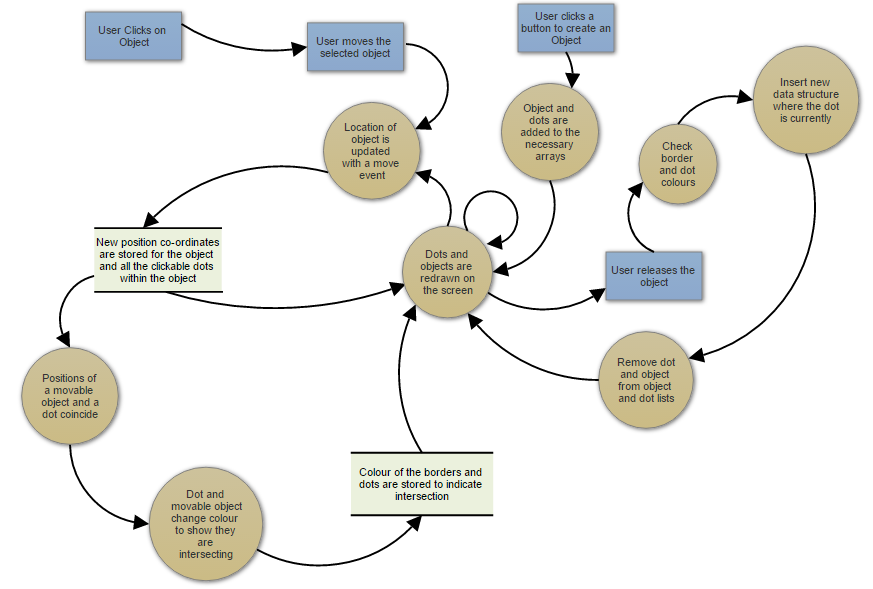
\includegraphics[angle=270, scale=0.8]{NaturalDeduction}
\caption{Data Flow Diagram on how Drag and Drop works}
\label{fig:NaturalDeduction}
\end{figure}

\section{Architecture Design}

This section describes the structure and layout of the program. It describes in detail how things will be done in the software and how all of the requirements will be met. It will outline how different sections of the program will interact and work together to create successful software without going into all the details of individual algorithms.

There will be a very simple file structure to the program. The site will be run from a HTML file. Embedded in this will be 2 Javascript files, one which will be a linear tutorial for users to go through and a second file that will allow the user play the game. A Cascading Style Sheet (CSS) file will be in charge of the design of the program which will make it look visually appealing and align elements in the correct places. CSS files describes the presentation of a HTML file. These four files will contain everything that is needed to run the project. The two Javascript files will contain all of the logic of the program and have all the algorithms needed to draw the objects and to work out all of the dragging and dropping.  

The tutorial file will be where the user presses a button to reveal more of the tutorial, explaining the basic techniques to the user so they can gain skills and knowledge. This will have the same layout and style as the main game which the user can interact with, so that the user will be familiar with what they must do when they have to make their own solutions. Each part will be hidden or visable as the tutorial progresses. As the user finishes this tutorial, they will automatically be transferred to the page where the user can play and interact with the game and fully play it.

The main Javascript file will contain many functions which all have specific tasks. All of these functions will link together to make the key logic structure of the software. Keeping the functions small and specific will make the code more maintable and easier to read. It will also help when scaling the software and increasing its capabilities.

The three basic functions needed for dragging and dropping will be for when the mouse is clicked down, when the mouse is moved and when then mouse is released. Whilst these are the main functions, other tasks will be in seperate functions and called from these functions.

When the left click is pressed down, the function needs to determined whether the location of the mouse is over any of the drag and droppable objects on the screen.  If it is over an object then this should be the current object selected.

When an object is selected then the function for moving the mouse will be active. This function will need to continuously update by using a timer. This will make sure the location of the dragged object is correctly represented when the mouse is clicked down. This function must also recognise if the active object that is being moved has the same position as any of the other objects on the screen. If it does, then this function must react accordingly.

Finally, when the mouse is released any appropriate actions needed will actually be confirmed. This could be the joining together of two objects, the deletion of objects or possibily other interactions. It will also release the current object so the software recognises that no object is now selected to be moved.

Some of the main functions that will need to be called from these functions are as follows:

\begin{itemize}
\item{A deletion function which will remove both the object that can be dragged and the dots associated with it}
\item{A function that will check whether an object is being dragged onto another one}
\item{Functions that will concatenate formulas and proofs based on what area of the proof was dragged on to}
\end{itemize}

While these functions will be called by an event, (a mouse click or movement) there also needs to be functions that will render the proof continously so that the user gets a good experience from dragging and dropping items and it is without lag.

A drawing function must be called periodically. This can be done that from an inital function that will set up the environment, create the canvas and set the correct level. The initial function will be called on startup so the canvas is always present when the application is first loaded.

The re-drawing function will have to cycle through all the objects and draw them individually. If the proof is a statement which will be represented as a string, it will need to be rendered differently to if it is a proof structure, where multiple layers will need to be drawn and the box size changing respectively. For doing each of these things there will be a different function. Within the drawing function there will be a number of library functions used to draw text, align the text correctly and change the colours of text and borders.

Users will need to create their own proofs from scratch and they will do this by having a number of buttons available to them which will then call a function in the Javascript to create the desired object. The buttons will be created in the HTML file and will call a function in the Javascript which is connected to that button. There will be javascript functions for different proof shapes, variables and connectors such as implication and negation.

The last set of functions that will be important for the game to work successfully are functions that determine the level information and that will verify whether answers are correct. A function will hide and show certain information depending on the level that a user is on. Removing certain elements that is not needed for a level makes it easier for a user to know what to do. Also, certain hints and tips can be shown on various levels depending on what the user has learnt to do. This function will neccessarily make sure the user is not overwhelmed with content and only the parts they need to use are included in each level.

A final function will be a verification check to see if what the user has created is a valid solution, and whether this solution is correct. This will be a comparison algorithm between an ideal, valid solution for a particular level and the user's attempt at the level. This algorithm should take into account different orders that the proof can be presented in, which will make it more complex than just a simple comparison algorithm.

\section{Interface Design}

\subsection{Design Principles}

Designing the visual representation that the user will be presented with is crucial to any design process. Making something that is aesthetically pleasing to look at and also easy to navigate can be just as important to the user as the functionality of the software. Software which has the capabilities to do a lot and is computationally good but has a poor user interface can really be detrimental to user experience so thinking about how users interact with the software needs to be concidered.

The users will be teenagers and young adults. Realising the users who will mainly play the game will affect how it is designed. This age group are technologically savvy and are used to frequently using touchscreens where swiping and dragging is commonplace. While this project will not be using touchscreens, understanding that the audience does not need to be patronised about how to use a computer is important. By keeping a simple and straightforward design, the users can focus their time on learning Natural Deduction and less time navigating many menus. Users will achieve the levels quicker with a declutted screen with only the necessary features displayed.

Consistancy is also crucial when designing a user interface. Each level should have the same layout, the canvas in the same place, the buttons in the same place. By creating this consistancy, the user will familiarise themselves with the structure and layout, and they will know what to do, for example, create a new variable object, or what is required when they need delete everything on the screen. The tutorial is especially important to have the same format as the main game, because this will be the first time a user will see the game and the interface. This will be when most of the learning of the interface will take place.  

The interface should be designed so if the user has not learnt correct way to use the interface, they should be notified what they have done correctly or incorrectly. This instant user feedback will not only help the user how to use the interface correctly, but also stop future similar mistakes. Users should not be in a position that they are puzzled in what is going on and therefore should be constantly told if an action they have performed is invalid.

Even if an action is valid, sometimes the user is mistaken in their action. Users ideally would not want to start again if they make one mistake. Some way of rectifying a mistake will be beneficial for overall user experience. Creating a user interface which takes into account mistakes will hopefully be used much more that requires a user to go through a long process of creating their proof again.
  
Crucially, the user must feel they are in control of the system at all times. They will feel comfortable when what they expect to happen does happen and this is helped by the consistant clear design. If the user doesn't encounter any suprises and is not confused then the design is fit for purpose.

\subsection{User Designs}

Taking into account all of these attributes, it is important to envisage and plan what you want the ideal user interface design to look like before implementing it. Four designs for a potential user interface were suggested for different elements of the game. Advantages and disadvantages of each design are outlined below: 

\subsubsection{Basic Level Design}
\centerline{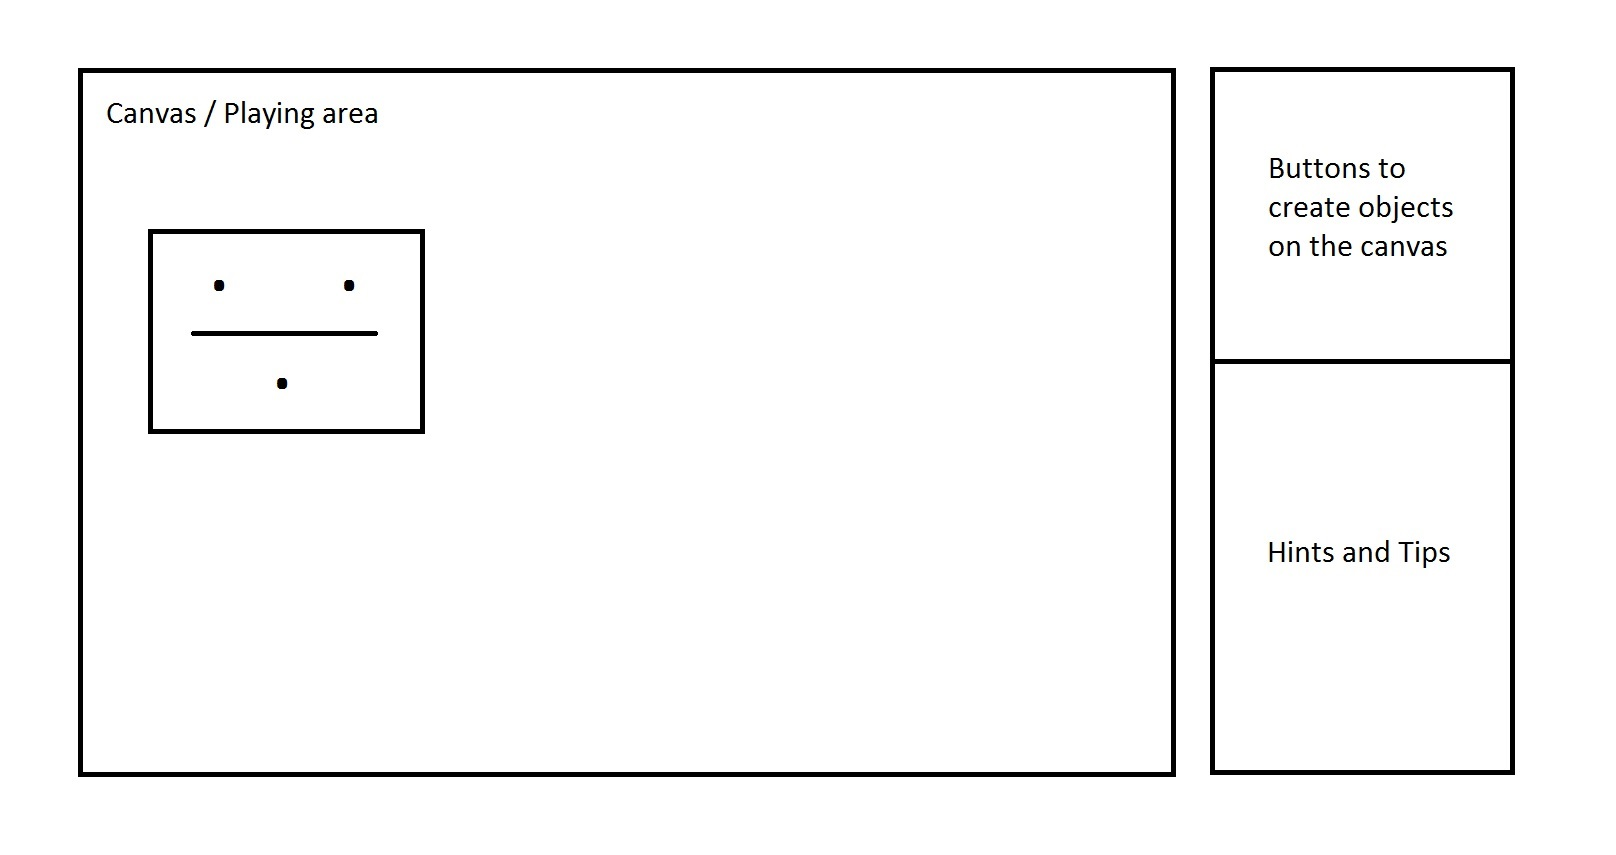
\includegraphics[angle=0, scale=0.3]{Design1}}

This first design is the basic layout of the game. It keeps a clean, simple design where every box has a very different purpose. The canvas is detached from the rest of the game to indicate the area you can drag and drop from. This will be outlined in the tutorial page. The box that is placed on the canvas is a proof structure which appears once a proof structure button is pressed in the top right box where the buttons are contained. Hints that the user can use to remind themselves what they have learnt are placed in the bottom right box and there may be an option to toggle hints on and off, so the user only gets the help if they need it.

A waste bin and brackets will be placed in the corners of the canvas so users can drag there elements to either the bin or brackets, depending on what the user wants to do. By keeping the core design to these simple elements, it will make the user feel in control because there are no complicated menus to navigate, making the user experience smooth. 

\subsubsection{Pop up boxes for level introduction}
\centerline{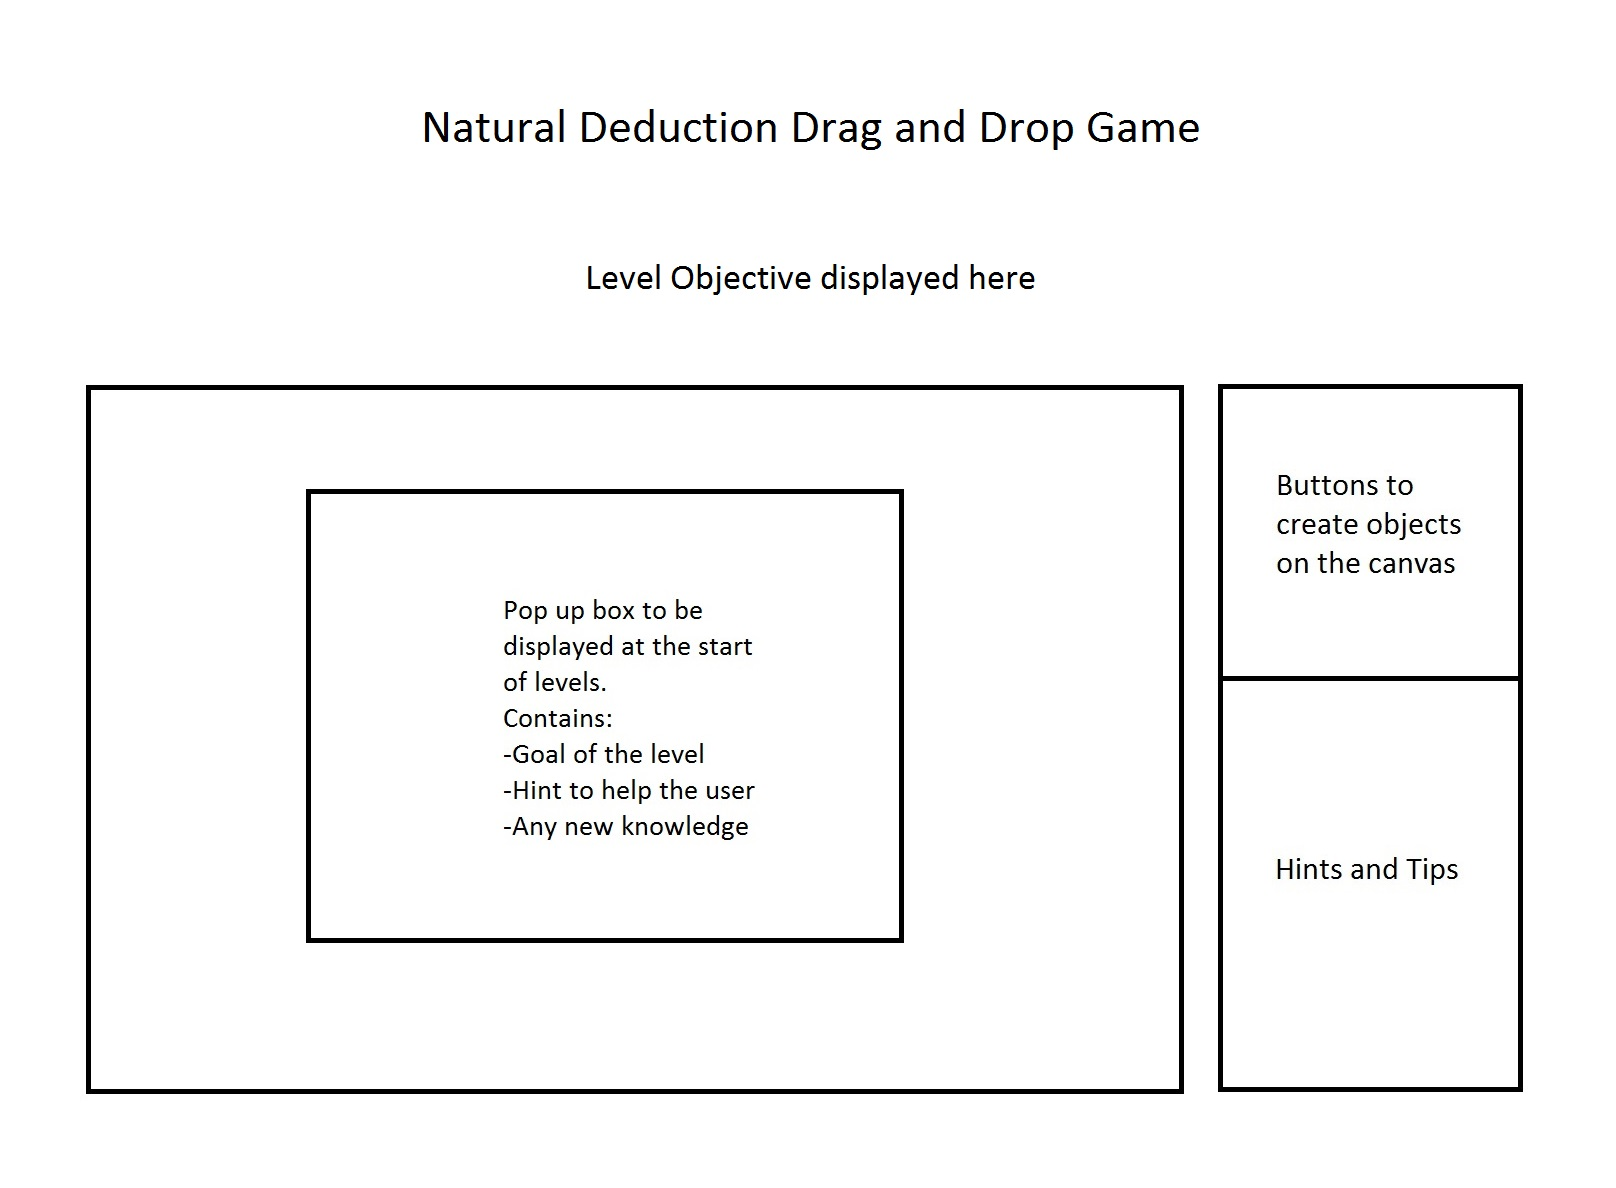
\includegraphics[angle=0, scale=0.3]{Design2}}

The second design screen understandably takes a very similar format of the first screen. All of the boxes are in the same place which keep continuity. This screen is to demonstrate what is presented to the user when they start a new level. All of the boxes including the canvas and the buttons will remain visable but not clickable whist the pop up is active on the screen. The pop up will show the proof that the user needs to make. Pop ups will also be used to introduce new content to the user that they can then use in future levels. The user will have to click a button on the pop up to dismiss it and then they can play the level, like shown in the first design.

\subsubsection{Multiple lines of proof and other objects on the canvas}
\centerline{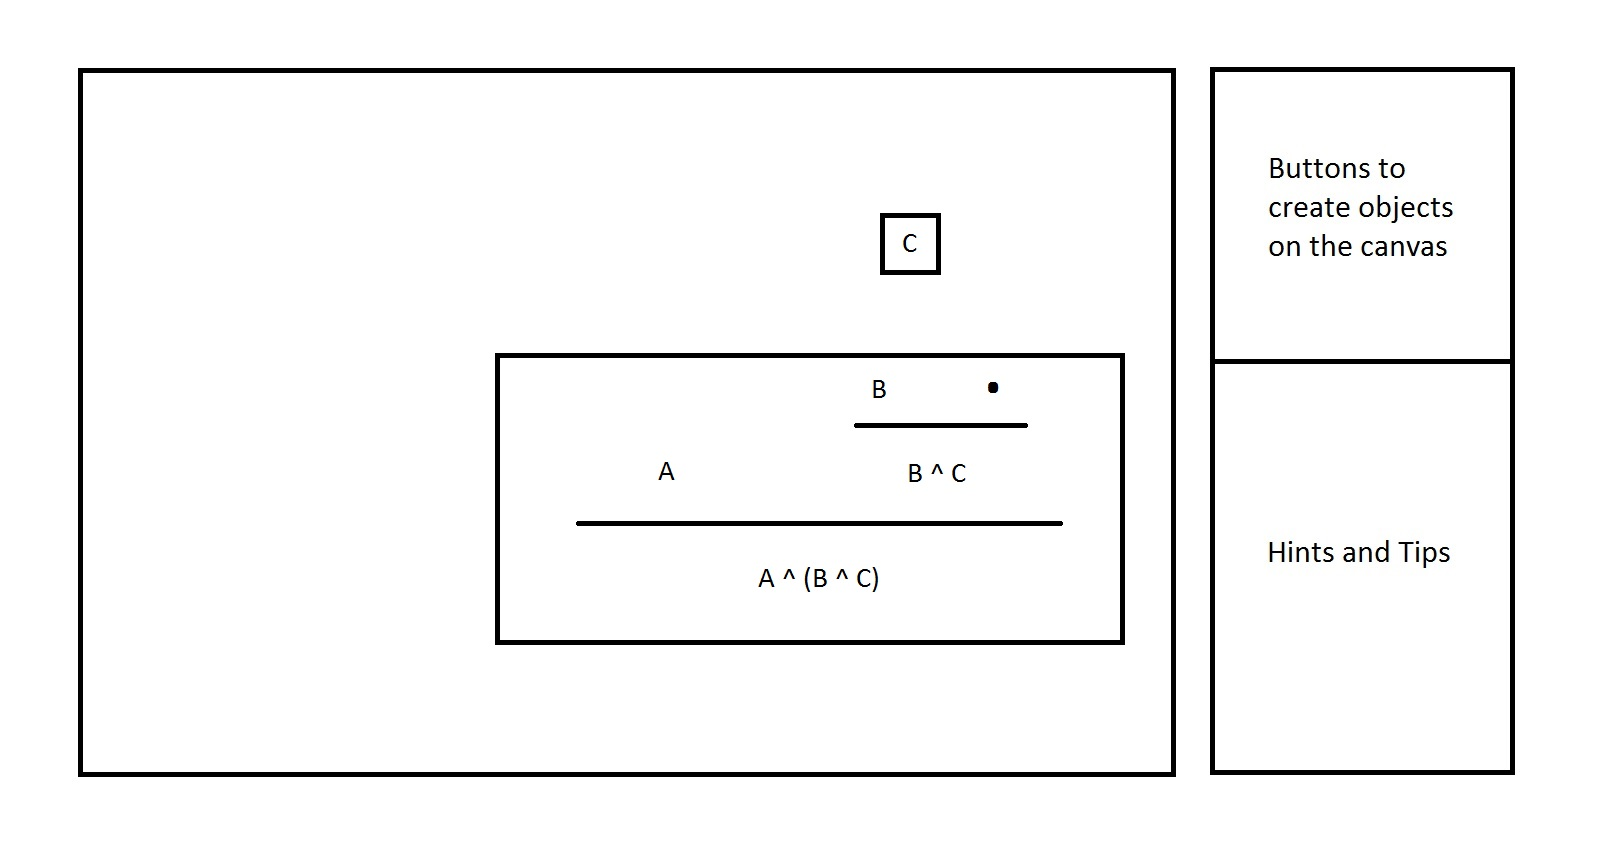
\includegraphics[angle=0, scale=0.3]{Design3}}

The third screen displays how a user will build a proof of muliple layers. Once the user drags proofs together then the software will automatically detect the new form the proof needs to be drawn and will be rendered differently. The only positions that users will be able to drag onto the proof will be where the dots exist. In the design, the user would drag the 'C' element onto the remaining dot to complete the proof.